
\section{Shaper CR-RC}\label{sec:shaper}
In questa sezione si realizza il secondo modulo della catena elettronica: si tratta di un circuito (detto shaper) per modificare la forma del
segnale in uscita dal preamplificatore (rendendolo simile ad una gaussiana) e
per ridurne la durata. Si vuole in particolare evitare che si verifichi il fenomeno di ``pile up'' del segnale, che si manifesta in situazioni di alte
frequenze di acquisizione in cui i segnali possono sovrapporsi e compromettere così l'informazione da acquisire.
Si studia inoltre la risposta in frequenza dello shaper e infine si
osserva e corregge l'effetto di Pole-Zero.

%------------------------------------------------
%	Configurazione Sperimentale
%------------------------------------------------

\subsection{Configurazione Sperimentale}\label{sec:shaper_config}
\begin{wrapfigure}{r}{0.5\textwidth}
  \centering
  \begin{circuitikz}[scale=0.7, transform shape, use fpu reciprocal]
     \draw(0,0) node[ground]{}
      (0,2) to[american voltage source,l=$V_{gen}$](0,0);
      \draw(0,2)-- (1,2) to[C,l_=$C_{sh1}$,font=\boldmath] (4,2)
          (4,2) to[R,l=$R_{sh1}$,font=\boldmath] (4,0) to (4,0) node[ground]{};
      \draw(6,2.5) node[op amp] (OA2){$OA_{2}$}
        (OA2.+)-- (4,2)
        (OA2.-)-- (4.5,3)-- (4.5,4)-- (7.5,4)-- (7.5,2.5)
        (OA2.out)-- (8,2.5) to[R,l=$R_{sh2}$,font=\boldmath] (10,2.5)
          (10,2.5) to[C,l_=$C_{sh2}$,font=\boldmath] (10,1) node[ground]{}
       (10,2.5) to[short,-*,l=$V_{out}$,font=\boldmath] (11,2.5);
    \end{circuitikz}
  \caption{\footnotesize Schema a variabili concentrate del circuito shaper $CR-RC$.}\label{fig:shaper-circuito}
\end{wrapfigure}
Si assembla il circuito in Figura~\ref{fig:shaper-circuito} utilizzando due capacità uguali
$C_{\text{sh1}}$, $C_{\text{sh2}}$ e due resistenze
uguali $R_{\text{sh1}}$,$R_{\text{sh2}}$, i cui valori,
misurati col multimetro, vengono riportati nella Tabella~\ref{tab:shaper_misure}.
Si usa il secondo amplificatore operazionale incluso nello stesso integrato
TL082 utilizzato per il preamplificatore come buffer per disaccoppiare i due stadi
$C_{\text{sh1}}R_{\text{sh1}}-R_{\text{sh2}},C_{\text{sh2}}$. In un primo momento si inserisce in
ingresso un'onda quadra di bassa frequenza per simulare un preamplificatore
ideale che mantiene il segnale per un tempo indefinito e, dopo aver confrontato la risposta del circuito con le aspettative
teoriche e le simulazioni, si inserisce come ingresso dello shaper
l'output del preamplificatore operazionale.
\begin{table}[h]
\centering
\setlength{\tabcolsep}{10pt}
\begin{tabular}{ |c|c|c|  }
\hline
\multicolumn{3}{|c|}{Misure dirette dei componenti del circuito} \\
\hline
Label      & Valore & F.S.\\
\hline
$R_{\text{sh1}}$ & $100.2 \pm 0.5\kOhm$ & $200\kOhm$ \\
$R_{\text{sh2}}$ & $100.1 \pm 0.5\kOhm$ & $200\kOhm$ \\
$C_{\text{sh1}}$ & $0.102 \pm 0.003\nF$ &$2\nF$ \\
$C_{\text{sh2}}$ & $0.103 \pm 0.003\nF$ &$2\nF$ \\
\hline
\end{tabular}
\caption{\footnotesize Si mostrano in tabella i valori e le incertezze delle componenti usate
  per la realizzazione dello shaper, misurati con il multimetro Tenma. È stato riportato anche il fondo scala usato.}\label{tab:shaper_misure}
\end{table}

%------------------------------------------------
%	Analisi del circuito
%------------------------------------------------

\subsection{Analisi del circuito}\label{sec:shaper_analisi}
Dai valori riportati in Tabella~\ref{tab:shaper_misure} si ottengono due
stime dello shaping time $\tau_{sh1}=10.2\pm 0.3 \us$ e
$\tau_{sh2}=10.3\pm 0.3 \us$.
Vista l'ottima compatibilità, si procede col calcolare la media pesata  tra i due valori $\langle \tau_{sh}\rangle = 10.26\pm 0.14 \us$.
Assumendo ideale l'amplificatore operazionale e risolvendo il circuito
nell'ipotesi $\tau_{sh1}=\tau_{sh2}=\tau_{sh}$, si ottiene le funzione di trasferimento
\begin{align}
  A(s)=\frac{1}{\tau_{sh}}\,\frac{s}{{(s+\frac{1}{\tau_{sh}})}^{2}}
\end{align}
da cui si prevede che la risposta a un segnale di ingresso a gradino sia
\begin{align}
  V_{\out}=\frac{V_{\inp}}{\tau_{\sh}}\, t\, e^{-\frac{t}{\tau_{\sh}}}
\end{align}
Essa presenta una forma simile ad una gaussiana di larghezza proporzionale allo shaping time
$\tau_{\sh}$ e ha massimo
\begin{align}
  V_{\out}^{\text{max}}& =V_{\inp}/e
  &
    t_{\text{max}}&= \tau_{sh}
\end{align}
Dalla funzione di trasferimento si deduce inoltre che il circuito si comporta
come un derivatore
\begin{wrapfigure}{r}{0.5\textwidth}
  \centering
  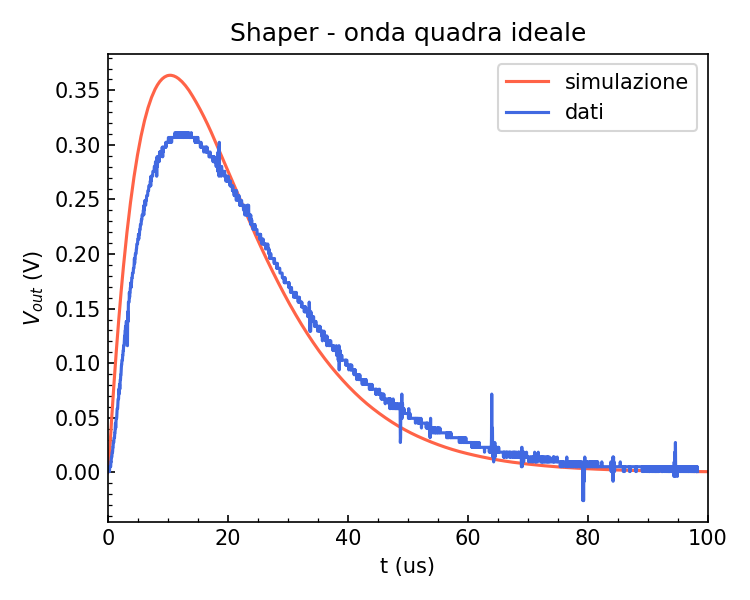
\includegraphics[width=0.48\textwidth]{../shaper/images/grafico_esp}
  \caption{\footnotesize{Risposta dello shaper ad un'onda quadra ideale.}}
\label{fig:shaper_id}%-----------------------------
\end{wrapfigure}
\noindent a basse frequenze e che, dopo una breve regione di midband, si comporta come
un integatore a frequenze alte.
Per verificare la corretta configurazione dell'apparato sperimentale si acquisicono
delle prime misure esplorative: si imposta il generatore in modo da erogare un'onda quadra
di frequenza $100\Hz$ e ampiezza $1\V$ per simulare un preamplificatore ideale. Utilizzando
i cursori di tensione e di tempo dell'oscilloscopio, si misura il massimo della tensione (rispetto alla baseline) in uscita, l'ampiezza dell'onda quadra in ingresso e lo shaping time.
I risultati delle misure e le aspettative teoriche sono riportate in Tabella~\ref{tab:shaper_misure_osc}, da cui si evidenzia una forte incompatibilità sia per
la tensione massima che per lo shaping time. Si attribuisce questa discrepanza alla non idealità dei componenti del circuito e alla presenza di capacità parassite dovute ai cavi e alla breadboard che portano ad una sottostima del tempo caratteristico. Questa anomalia risulta ancora più
evidente dal grafico in Figura~\ref{fig:shaper_id}, in cui viene confrontato il segnale rilevato
dall'oscilloscopio con la simulazione LTspice.

\begin{table}[h]
\centering
\setlength{\tabcolsep}{10pt}
\begin{tabular}{ |c|c|c|  }
\hline
\multicolumn{3}{|c|}{Misure oscilloscopio} \\
\hline
\multicolumn{3}{|c|}{$V_{\inp,\text{sp}}= 0.98 \pm 0.02\V$} \\
\hline
Misura      & Aspetattiva & Compatibilità\\
$V_{\out,\text{sp}}^{\text{max}}= 0.315\pm 0.006\V$    & $V_{\out,\text{th}}^{\text{max}}= 0.362\pm 0.007\V$  & $\lambda=5.0$\\
$\tau_{\sh,\text{sp}}= 11.7 \pm 0.4\us$  & $\tau_{\sh,\text{th}}= 10.3\pm 0.3\us$ & $\lambda=12.8$\\
\hline
\end{tabular}
\caption{\footnotesize{Si mostrano in tabella i valori e le incertezze delle misure effettuate con l'oscilloscopio. In particolare si riporta la tensione massima sperimentale $V_{\out,\text{sp}}^{\text{max}}$, lo shaping time $\tau_{\sh,\text{th}}$ e la misura dell'ampiezza
  dell'onda quadra in ingresso. Si riportano anche le aspettative teoriche e si calcola la compatibilità.}}\label{tab:shaper_misure_osc}
\end{table}

%------------------------------------------------
%	Risposta in frequenza dello shaper
%------------------------------------------------

\subsection{Risposta in frequenza dello Shaper}\label{sec:shaper_bode}
In questa sezione si studia la risposta del circuito a segnali sinusoidali di ampiezza
$1\V$ e frequenze comprese tra $0.1\kHz$ e $100\kHz$. Si registrano quindi per ogni
frequenza campionata le tensioni di ingresso e di uscita utilizzando i cursori verticali
dell'oscilloscopio. Infine, si realizza il grafico di Bode e da esso si stima la frequenza relativa al polo della funzione di trasferimento.

\subsubsection{Analisi Dati}\label{sec:shaper_bode_analisi}

Per il calcolo della funzione di trasferimento e per le considerazioni sulla sua incertezza
si rimanda alla Sezione~\ref{sec:preamp_bode}. Si mostra in Figura~\ref{fig:shaper_bode} il grafico di Bode
confrontato con una simulazione. Si nota subito come il circuito si comporti come previsto
nella Sezione~\ref{sec:shaper_analisi}: per basse frequenze funziona come derivatore e presenta
una regione ad alta frequenza in cui integra. Tuttavia, sono evidenti numerose discrepanze con la simulazione, soprattuto a basse e alte frequenze. Questo non sorprende considerando gli scarsi
risultati già ottenuti nella sezione precedente e soprattutto osservando l'ampio range di
frequenze analizzato.
In Figura~\ref{fig:shaper_bode} vengono riportate anche due interpolazioni lineari: una per la
regione di derivazione (in blu) e una per quella di integrazione (in rosso).
L'intersezione delle due rette fornisce una stima della frequenza relativa
al polo doppio della funzione di trasferimento dello shaper $f_{\text{fit}}=12.3\pm 0.3 \kHz$,
compatibile con l'aspettativa $f_{\text{sp}}=13.6\pm 0.5\kHz$, ottenuta utilizzando la stima sperimentale
dello shaping time riportata in Tabella~\ref{tab:shaper_misure_osc} ($\lambda=2.3$). Risulta invece incompatibile ($\lambda=8.4$) con la frequenza
$f_{\text{th}}=15.5\pm 0.2\kHz$, ricavata a partire dallo shaping time teorico.
\begin{figure}[h]
\centering
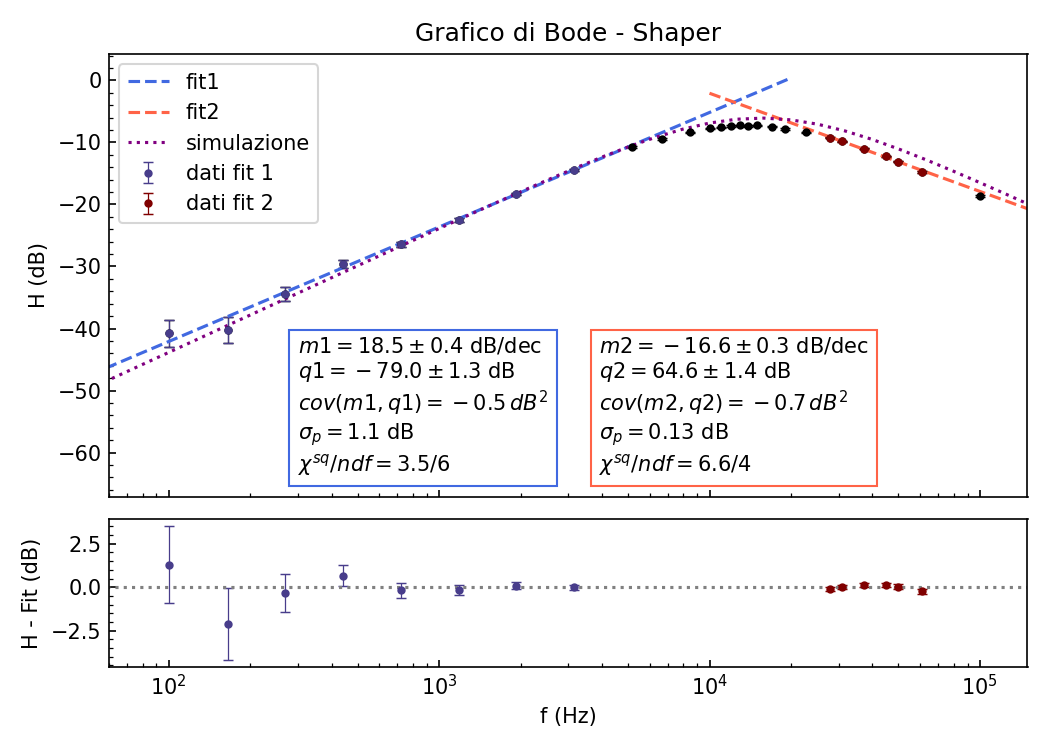
\includegraphics[width=0.8\textwidth]{../shaper/images/fit_bode}
\caption{\footnotesize Grafico di Bode dello shaper $CR-RC$ confrontato con la simulazione LTspice. In basso vengono mostrati i residui delle due interpolazioni lineari.}\label{fig:shaper_bode}
\end{figure}

%------------------------------------
%------------------------------------------------
%	Shaper con Pole-Zero
%------------------------------------------------

\subsection{Shaper con compensazione Pole-Zero}\label{sec:shaper_pz}

Si mette ora in input allo shaper l'output del preamplificatore: in questo modo non si ha più
un'onda quadra ideale in ingresso, ma un segnale che cresce linearmente e caratterizzato da
una discesa lenta. Si osserva quindi il fenomeno di undershoot, per cui la tensione prima
di raggiungere asintoticamente la baseline diventa negativa fino a raggiungere
il minimo
$V_{\text{undershoot}}\approx-25\,\si{m\volt}$, per poi risalire
lentamente. Questo vanifica parzialmente l'effetto di riduzione della durata
del segnale dello shaper e quindi si cerca di rimediare tramite
il metodo di compensazione Pole-Zero: aggiungendo una resistenza $R_{\text{pz}}$ in parallelo al condensatore $C_{\sh 1}$, il segnale che
arriva all'ingresso dell'$RC$ è dato da
\begin{align}
  V_{1}(s)&=\frac{V_{\inp}}{s+\frac{1}{\tau_{\text{pre}}}}\frac{s+\frac{1}{\tau_{\text{pz}}}}{s+\frac{1}{\tau_{\parallel}}}
  &
    \text{con }& \begin{cases}
      \tau_{\text{pz}}=R_{\text{pz}}\,C_{\text{sh1}}\\
      \tau_{\parallel}=R_{\parallel}\,C_{\text{sh1}}=\left(\frac{1}{R_{1}}+\frac{1}{R_{\text pz}}\right)^{-1}\,C_{\text{sh1}}
    \end{cases}
\end{align}
Scegliendo la resistenza di Pole-Zero tale che valga la relazione $\tau_{\text{pz}}=\tau_{\text{pre}}$, si annulla l'effetto del polo del preamplificatore,
responsabile del fenomeno di undershoot. Deve quindi valere $R_{\text{pz}}=1.51\pm 0.06\MOhm$ e, osservando che
tale valore è molto più grande delle resitenze $R_{\sh 1}$ e $R_{\sh2}$, segue che $\tau_{\parallel}\approx \tau_{\sh 1}$
e si ottiene approssimativamente lo stesso polo del circuito $CR$ non modificato. Si aggiungono quindi al circuito due resistenze in serie in modo
da ottenere la resistenza equivalente
\begin{align}
  R_{\text{pz,sp}}&= (0.558\pm0.002)\MOhm + (1.009\pm0.005)\MOhm = (1.567\pm 0.006) \MOhm
\end{align}
che presenta un'ottima compatibilità col valore richiesto ($\lambda=0.9$).
In Figura~\ref{fig:shaper_undershoot} viene mostrato il segnale di uscita dell'oscilloscopio prima e
dopo la correzione di Pole-Zero. Si mostra anche il fenomeno di interferenza
anticipato nella Sezione~\ref{sec:preamp_config_sperim} e che ha dominato questa parte dell'esperienza.
Il segnale risulta infatti visibilmente ``sporco'', complice anche il fatto
che le tensioni in gioco sono prossime ai limiti imposti dalla precisione
del Picoscope. Si nota comunque un discreto accordo con le simulazioni e
dopo $10\, \tau_{\text{sh1}}$ la tensione risulta compatibile con la baseline, confermando, per quanto possibile date le circostanze, una
corretta compensazione di Pole-Zero.
%------------------------------------
\begin{figure}[h]
\centering
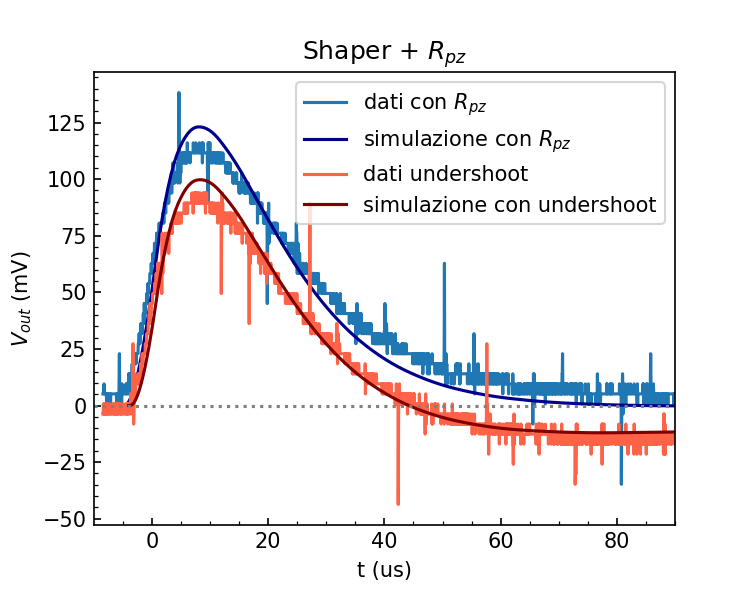
\includegraphics[width=0.6\textwidth]{../shaper/images/undershoot}
\caption{\footnotesize{Si mostrano in grafico le simulazioni e i segnali rilevati dall'oscilloscopio in configurazione con undershoot e con compensazione di Pole-Zero. Si osserva anche il fenomeno di forte interferenza che ha complicato l'acquisizione delle misure in quest'ultima sezione relativa allo shaper.}}\label{fig:shaper_undershoot}
\end{figure}
